% !TEX TS-program = LuaLaTeX
\documentclass[10pt, oneside, a4paper]{article}

\usepackage[T1]{fontenc}
\usepackage{lmodern}
\usepackage{xcolor}
    \definecolor{gray} {HTML}{363636}
    \definecolor{red}  {HTML}{950009}
    \definecolor{green}{HTML}{0E610A}
    \definecolor{blue} {HTML}{020069}
\usepackage{fontspec}
    \setsansfont{Arial}
\usepackage{amsmath}
\usepackage{titlesec}
    \titleformat*{\section}      {\color{gray}\large\bfseries\sffamily}
    \titleformat*{\subsection}   {\color{gray}\large\bfseries\sffamily}
    \titleformat*{\subsubsection}{\color{gray}\large\bfseries\sffamily}
\usepackage{geometry}
%   \geometry{showframe}
    \geometry{scale={0.75,0.85}}
%\usepackage{pgfplots}
%    \pgfplotsset{compat=newest}
\usepackage{siunitx}
    \sisetup{locale=FR}
\usepackage{graphicx}
\usepackage{caption}
    \captionsetup{labelfont={bf,sf,color=gray}}
\usepackage{pdfpages}


% Keep lasts
\usepackage[french]{babel}
    \frenchsetup{SmallCapsFigTabCaptions=false}
\usepackage[expansion]{microtype}
\usepackage[luatex, backref]{hyperref}
    \hypersetup{unicode, colorlinks, breaklinks, urlcolor=red,
                bookmarksopen, bookmarksnumbered}

\renewcommand{\UrlFont}{\small}
\renewcommand{\arraystretch}{1.1}
\newcommand{\important}[1]{\textbf{\textsf{\color{gray}{#1}}}}
\setlength{\parskip}{2mm}
\newcommand\AtUpperLeftCorner[3]{%
\put(\LenToUnit{#1},\LenToUnit{\dimexpr\paperheight-#2}){\blap{#3}}%
}

\begin{document}

\begin{titlepage}
    \centering
    \includegraphics[width=0.5\textwidth]{image/logo-ecam.png}\par
    \vspace{1cm}
    
    \rule{\linewidth}{1.5pt}%
    \vspace{5mm}
    {\rm\sffamily\LARGE Rapport de bureau d'étude\par}
    \vspace{3mm}
    {\sffamily\bfseries\LARGE Réalisation d'un amplificateur de classe D\par}
    \vspace{5mm}
    \rule{\linewidth}{1.5pt}%
    \vspace{1.5cm}
    
    {\Large%
        \begin{minipage}[t]{0.35\linewidth}
            \centering
            Alexis~\bsc{Nootens} \\[1mm]
            \href{mailto:16139@student.ecam.be}{16139@student.ecam.be}
        \end{minipage}
        \begin{minipage}[t]{0.35\linewidth}
            \centering
            Thomas~\bsc{Anizet} \\[1mm]
            \href{mailto:14164@student.ecam.be}{14164@student.ecam.be}
        \end{minipage}
    \par}
    \vspace{1.5cm}
    
    {\Large%
        ECAM Brussels             \\[1mm]
        Promenade de l'Alma 50    \\[1mm]
        1200 Woluwe-Saint-Lambert \\[1mm]
        Belgique
    \par}
    
    \vfill
    {\Large\today\par}
\end{titlepage}

%%%%%%%%%%%%%%%%
\tableofcontents
\newpage

%%%%%%%%%%%%%%%%%%%%%%%
\section*{Introduction}
    \pdfbookmark[1]{Introduction}{sec:intro}
Après avoir étudié la théorie derrière le transfert de puissance en électronique,
nous avons mis à l'épreuve nos acquis théoriques dans un cas pratique en réalisant un circuit d'amplification de signaux audio analogiques.
Ce circuit d'amplification appartient à la classe D, une classe exploitant la connaissance de l'électronique de puissance, pour minimiser les pertes d'énergies aux étages d'amplification.
Ce document reprend notre réalisation et notre analyse du circuit.


%%%%%%%%%%%%%%%%%%%%%%%%%%%%%%%%
\section{Hypothèses de départ}
    \label{sec:hypothese}
Avant de s'attaquer au problème, définissons l'environnement dans lequel nous allons travailler tel que la nature du signal reçu en entré.
Notre amplificateur doit être conçu pour les signaux audio ;
les signaux audio sont produit par un module convertisseur analogique-numérique (sigle CAN, ou DAC en anglais).
Leur tension est asymétrique entre \num{0} et une référence observée habituellement à \SI{2048}{\milli\volt} et leur fréquence varie entre \num{20} et \SI{22000}{\hertz}~\cite{heffner2007hearing}.
Nous supprimerons donc les composantes fréquentielles hors de ces bornes par des filtres passe-haut et passe-bas distincts.


%%%%%%%%%%%%%%%%%%%%%%%%%%%%%
\section{Circuit amplificateur}
Le circuit réalisé repose sur deux modules pour amplifier le signal d'entré :
un convertisseur analogique-numérique de type Sigma-Delta, et un contrôleur de transistor MOSFET.
La mise en série de ces deux modules permet de créer un amplificateur de classe D.
Les sous-sections \ref{sec:sigmaDelta} et \ref{sec:classeD} définissent le principe derrière chaque module et évoquent leur raison d'être.


\subsection{Modulation Sigma-Delta}
    \label{sec:sigmaDelta}
Il existe une évolution des méthodes de modulation en pleine onde.
La plus simple est la modulation de largeur d'impulsion, MLI.
% Modulation de Largeur d'Impulsion
Voici comment elle fonctionne : depuis deux états possibles de tension, haut et bas, une période d'impulsion nommée \tau, et une durée variable de tension haute nommée $t$, le signal respecte la condition suivante : $0 \leq t \leq \tau $, soit $t \div \tau \in [0,1]$.
L'information modulée se situe dans le rapport de durée tension haute sur durée d'impulsion.
La donnée nécessite d'être transposée au préalable dans l'interval entre 0 et 1.
Cette modulation bénéficie de pouvoir être directement applicable comme commande d'un étage d'amplification en puissance.
Elle se traduit sans opération supplémentaire en commande complètement ouverte ou complètement fermée de transistor.

% Modulation Delta
Une évolution de la modulation de largeur d'impulsion est la modulation Delta.
Tandis que la MLI encode l'entièreté de l'information dans son rapport cyclique à chaque période, la modulation Delta n'encode que la différence (delta) par rapport à l'information précédente.
Les différences entre informations sont de taille plus petites que les informations entières.
Elles sont envoyées plus rapidement.
Ainsi, pour une période donnée, plus de delta pourront être envoyés que de cycles MLI complets.
Le modulateur fonctionnera à une fréquence plus élevée, suréchantillonnant le signal, ce qui réduit le bruit de quantification~\cite{gray1998quantization} par rapport à un modulateur MLI.

% Modulation Sigma-Delta
La modulation Delta connecte la sortie à l'entrée pour la différentier, c'est une rétro-action.
Un automaticien y reconnaîtra un contrôle en boucle fermée proportionnel, un régulateur P.
Cet automaticien saura également que ces régulateurs ont le défaut de toujours avoir un décalage entre la consigne et le signal de sortie désiré, nommé \og écart statique \fg{}.
Ce problème se résout en ajoutant un intégrateur avant la comparaison ; ce dernier maintient la dernière valeur comparu.
Cela devient un régulateur PI \og proportional-integral \fg{}.
Cette nouvelle modulation se nomme \important{Sigma-Delta}, puisqu'elle somme (\Sigma) les différences (\Delta).

Le schéma fonctionnel d'un circuit sigma-delta est présenté à la figure~\ref{fig:sigmaDelta}.
Voici son fonctionnement :
pour un signal d'entrée constant non nul, le différentiateur débute par soustraire le signal de sortie à l'entrée.
Si le système est reposé, la sortie est nulle et le signal d'entrée arrive pleinement à l'intégrateur.
L'intégrateur va introduire une temporisation dans le système ;
le signal à la sortie de l'intégrateur grimpe progressivement de manière monotone.
Ce signal arrive à l'entrée d'un comparateur qui retourne une tension soit maximale, soit minimale.
C'est ce signal binaire qui est réutilisé en rétro-action.
Le système va tenter de compenser le signal d'entrée avec la tension haute ou la tension basse.
Cette tension n'ayant pas de valeur intermédiaire, le système ne parviendra jamais à compenser le signal d'entré si celui-ci se trouve entre les bornes.
Le système est oscillant.
L'information modulée s'encode comme les différences entre cycle tension haute--basse.

\begin{figure}[tbp]
    \centering
    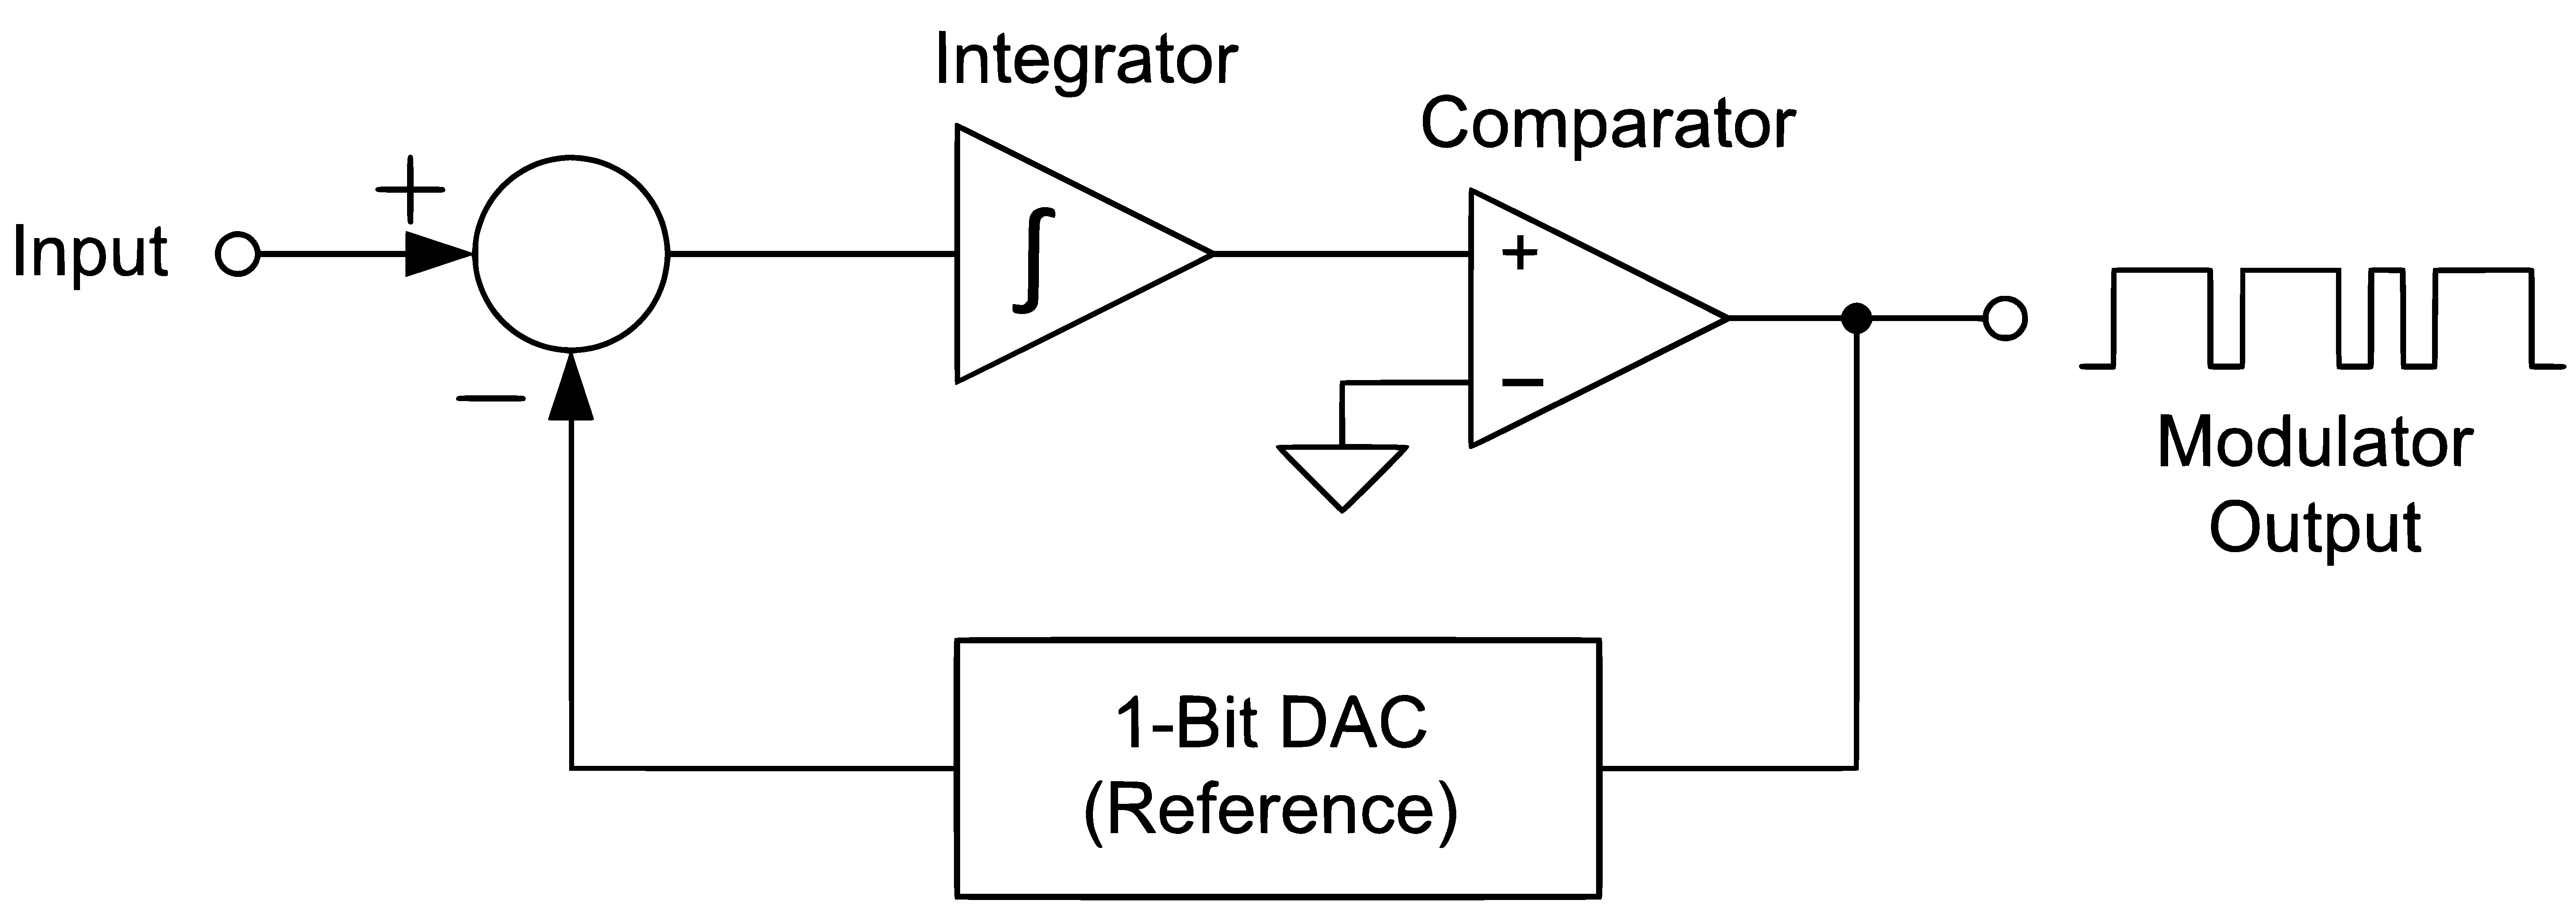
\includegraphics[width=0.7\textwidth]{eps/sigma-delta.eps}
    \caption{Schématique symbolique d'un modulateur \Sigma-\Delta.
    Le signal d'entrée \og Input \fg{}{} est de nature analogique.
    Le circuit agit en boucle fermée pour compenser la différence entre entrée et sortie.}
    \label{fig:sigmaDelta}
\end{figure}


\subsection{Amplificateur de classe D}
    \label{sec:classeD}
La famille des amplificateurs contient plusieurs divisions --- dénommées \og classes \fg{} --- selon la nature du signal en sortie.
Par exemples :
les amplificateurs de classe A sortent une tension sinusoïdale amplifiée sur les deux crêtes ;
les amplificateurs de classe B ne laissent sortir qu'une seule crête amplifiée du sinus.

Les amplificateurs de classe D imposent des tensions aux rails d'alimentation du circuit.
C'est du tout ou rien.
Ils sont composés de transistor MOSFET.
Les transistors MOSFET sont les favoris de l'électronique de basse puissance.
Ils peuvent travailler à haute fréquence (plusieurs dizaines de kHz) et leur résistance à la conduction en saturation \og $\text{R}_{\text{DS,ON}}$ \fg{} est très faible (une centaine de m\Omega{} dans les basses puissances)~\cite{irf2017mosfet}.
Cette propriété donne tout son intérêt à l'amplificateur de classe D.
En ouvrant ou fermant complètement les transistors pour les faire fonctionner dans leur zone saturée, on minimise la résistance de conduction.
Sachant que la perte en conduction est dû à l'effet joule, et que la puissance de l'effet joule se formule comme $P=RI^2$~\cite{griffiths1999introduction}.
Lorsque $R$, la résistance du transistor est minimale, la puissance $P$ perdue à la conduction est minimisée pour une courant $I$ donné~\cite{sente2017elec}.
Le principe de l'amplificateur de classe D est présenté visuellement à la figure~\ref{fig:classeD}.
Un filtre LC peut-être placé à la suite de l'étage d'amplification pour lisser le courant et la tension~\cite{wildi2005electrotech}.
Dans notre réalisation, nous considérons que le bobinage du haut-parleur lissera le courant et nous ne placerons pas d'inductance discrète.

\begin{figure}[tbp]
    \centering
    \includegraphics[width=0.5\textwidth]{eps/classe-d.eps}
    \caption{Schématique du principe de l'amplificateur de classe D.
    Le signal d'entré analogique est modulé en commande de commutation de transistor de puissance.
    Le signal amplifié se trouve à l'état $+\text{Vdd}$ ou $-\text{Vss}$ uniquement.
    Ce signal est ensuite lissé au travers d'un filtre LC pour retrouver des tensions intermédiaires.}
    \label{fig:classeD}
\end{figure}


%%%%%%%%%%%%%%%%%%%%%%%%%%%%%%
\section{Schématique du circuit}


%%%%%%%%%%%%%%%%%%%%%%%%%
\section{Dimensionnement}

\subsection{Filtre pré-amplification}
\subsubsection{Définitions}
À la section~\ref{sec:hypothese} : \og Hypothèses considérées\fg, nous avions considéré que la fréquence pouvait varier entre 20 et 20 000 Hz. Pour obtenir une telle bande passante, nous utilisons des \textbf{filtres}. Il existe 2 types de filtres selon les composants électroniques utilisés : 
\begin{itemize}
\item \textbf{Filtre passif} : Les filtres passifs sont réalisés avec des composants passifs : principalement des résistances, des inductances et des condensateurs. En général, ils ont un gain en puissance de l'ordre de 1.
\item \textbf{Filtre actif} : Les filtres actifs sont réalisés principalement avec des composants actifs: des transistors et des amplificateurs opérationnels. On retrouve également des condensateurs ainsi que des résistances. En général, ils ont un gain en puissance plus élevé.
\end{itemize}
Pour notre circuit, nous utilisons deux condensateurs, deux résistances ainsi qu'un amplificateur opérationnel : Il s'agit donc de filtres actifs. 

La \textbf{\textit{réponse fréquentielle}} d'un filtre correspond à l'évolution de son gain en tension en fonction de la fréquence. On peut observer la réponse fréquentielle à l'aide d'un \textbf{\textit{diagramme de Bode}}.
On définit 5 types de filtres selon leur réponse fréquentielle : \textit{passe-bas}, \textit{passe-haut}, \textit{passe-bande}, \textit{coupe-bande} et \textit{passe-tout}. Nous ne nous intéresserons cependant qu'aux filtres passes-bas, passe-haut et passe bande étant donné que ce sont les seuls utilisés dans le circuit.
\begin{description}
\item[Filtre passe-bande :] Dans un filtre passe-bande, une gamme spécifique des fréquences doit être passée alors que les autres fréquences sont bloquées. Par définition, ce filtre permet donc de réaliser ce que l'on désire, à savoir laisser passer les signaux dont la fréquence est comprise entre 20 et 20 000 Hz et bloquer ceux donc la fréquence se situe en-dehors de cette bande-passante. En pratique, nous utilisons un filtre passe-bas et un filtre passe-haut pour implémenter le passe-bande.
\item[Filtre passe-bas :] Un filtre passe-bas laisse passer toutes les fréquences depuis la fréquence nulle jusqu'à la fréquence de coupure et atténue toutes les fréquences supérieures à cette fréquence de coupure.
\item[Filtre passe-haut :] Un filtre passe-haut laisse passer toutes les fréquences supérieures à la fréquence de coupure et atténue toutes les fréquences depuis la fréquence nulle jusqu'à la fréquence de coupure.
\end{description}

Pour rappel, la \textbf{\textit{fréquence de coupure (notée $\text{fc}$}}) pour un filtre est la fréquence limite de fonctionnement utile de ce filtre. Ainsi, nous définissions deux fréquences de coupures : 
\begin{itemize}
\item \textbf{\textit{$\text{fc}$} du filtre passe-bas} : La fréquence de coupure du filtre passe-bas vaut 20 000 Hz. Cela signifie que ce filtre ne laisse passer que les signaux dont la fréquence est comprise entre la fréquence nulle et 20 000 Hz
\item \textbf{\textit{$\text{fc}$} du filtre passe-haut} : La fréquence de coupure du filtre passe-haut vaut 20 Hz. Cela signifie que ce filtre ne laisse passer que les signaux dont la fréquence est supérieure à 20 Hz.
\end{itemize}

\subsubsection{Circuits schématiques}
La figure 3 ci-dessous présente le circuit schématique de la partie pré-amplification et filtre reçu au cours. Le trajet emprunté par le signal est le suivant : le signal analogique d'entrée arrive sur la pin \textit{ININVA}. Étant donné la nécessité d'un filtre passe-haut, l'ajout d'un condensateur entre les pins \textit{ININVA} et \textit{ININVB} est inévitable. Une fois qu'il a traversé le condensateur, le signal traverse la résistance \textit{R14}. Nous retrouvons ensuite un amplificateur opérationnel avec rétro-action (\textit{C18} et \textit{R13}) dont la sortie, dénommé par \textit{OUTINV}, renvoie un signal filtré (fréquence comprise entre 20 et 20 000 Hz). À noter que la résistance \textit{R15} n'est pas employée.
Afin de mieux visualiser le circuit schématique de la partie pré-amplification et filtre, la figure 4 est disponible ci-dessous.

\begin{figure}
    \centering
    \includegraphics[width=0.5\textwidth]{image/schematique-all-1.jpg}
    \caption{Schématique de la partie pré-amplification et filtre de l'amplificateur classe D. 
             Le signal d'entrée analogique arrive sur \textit{ININVA}. Ce signal poursuit son chemin tout d'abord à travers le condensateur placé entre \textit{ININVA} et \textit{ININVB} et ensuite à travers la résistance \textit{R14}. On retrouve le signal filtré à la sortie de l'amplificateur avec rétro-action (\textit{C18} et \textit{R13}) soit \textit{OUTINV}. À noter que la résistance \textit{R15} n'est pas employée.}
\end{figure}

\begin{figure}
    \centering
    \includegraphics[width=0.5\textwidth]{image/schematique-all-2.jpg}
    \caption{Circuit schématique semblable à celui de la figure 3 et permettant de mieux visualiser la partie pré-amplification et filtre de l'amplificateur classe D.}
\end{figure}

Afin de mieux distinguer les filtres sur le circuit schématique de la figure 3, les figures 5 et 6 présentent respectivement le circuit d'un filtre passe-bas et d'un filtre passe-haut : 

\begin{figure}[htbp]
    \centering
    \begin{minipage}[c]{.46\linewidth}
        \includegraphics[height=110pt, width=0.9\textwidth]{image/filtre-passe-bas.jpg}
        \caption{Filtre actif passe-bas de l'amplificateur classe D.}   
    \end{minipage} \hfill
    \begin{minipage}[c]{.46\linewidth}
        \includegraphics[height=110pt, width=1.1\textwidth]{image/filtre-passe-haut.jpg}
        \caption{Filtre actif passe-haut de l'amplificateur classe D.}    
    \end{minipage}
\end{figure}

\subsubsection{Étude théorique}
	\label{sec:etudeTheorique}
Pour dimensionner les composants électroniques (résistances et condensateurs) des deux filtres de l'amplificateur classe D, nous avons procédé comme suit : 

\textit{N.B.} : Se référer à la figure 4 de la page 6 pour la notation des deux résistances ($R1$ et $R2$) et des deux condensateurs ($C1$ et $C2$).

\begin{description}
\item[Pour le filtre passe-bas :] Durant le laboratoire, nous avons commencé par dimensionner le filtre passe-bas. La fréquence de coupure doit se trouver aux environ de \SI{20}{\kilo\hertz}.
    \begin{enumerate}
        \item Prendre les formules théoriques permettant de calculer la fréquence de coupure et le gain de l'amplificateur. Ces formules sont les suivantes : 
            \begin{center} $f_{c}=\frac{1}{2*\pi*R_{2}*C_{2}}$ \end{center} 
            \begin{center} $A_{v}=\frac{-R_{2}}{R_{1}}$ \end{center} 
        \item Poser comme hypothèse que nous souhaitons un gain unitaire. Cela signifie que la valeur de la résistance R1 est égale à la valeur de la résistance R2. En effet : \begin{center} $A_{v}=\frac{-R_{2}}{R_{1}} = -1$ \end{center} 
        \item Fixer une valeur standard pour R2 et ré-écrire la formule permettant de trouver la valeur de C2. Nous avons pris une valeur standard de 8200 Ohm pour la résistance R2.
            \begin{center} $R_{1}= R_{2} = 8 200\Omega $ \end{center}
            \begin{center} $C_{2}=\frac{1}{2*\pi*R_{2}*f_{c}}$ \end{center} 
        \item Cherchant une valeur la plus standardisée possible pour le condensateur C2, nous devons ajuster la valeur de la fréquence de coupure dans la formule donnée précédemment. Ceci nous conduit à ajuster la fréquence de coupure à 19 400 Hz.
            \begin{center} $C_{2}=\frac{1}{2*\pi*8 200*19 400}= 1 nF$ \end{center} 
    \end{enumerate}
\end{description}

\begin{description}
\item[ Pour le filtre passe-haut :] La fréquence de coupure doit se trouver aux environ de 20 Hz. Nous connaissons déjà les valeurs standards des deux résistances R1 et R2 ainsi que du condensateur C2. Il nous reste donc à calculer la valeur standard du condensateur C1.
    \begin{enumerate}
        \item Prendre la formule théorique permettant de calculer la fréquence de coupure :
            \begin{center} $f_{c}=\frac{1}{2*\pi*R_{2}*C_{1}}$ \end{center} 
        \item Ré-écrire la formule permettant de calculer la valeur standard de C1 : 
            \begin{center} $C_{1}=\frac{1}{2*\pi*R_{2}*f_{c}}$ \end{center} 
        \item Connaissant la valeur de R2, nous trouvons la valeur de C1 en ajustant la valeur de la fréquence de coupure. Nous trouvons finalement une fréquence de coupure de 18 Hz. 
            \begin{center} $C_{1}=\frac{1}{2*\pi*R_{2}*f_{c}}=\frac{1}{2*\pi*8200*18} = 1uF $ \end{center} 
    \end{enumerate}
\end{description}

Le tableau ci-dessous reprend les valeurs calculées pour le filtre passe-bas ainsi que pour le filtre passe-haut :
\begin{figure}
    \centering
    \includegraphics[scale=0.65]{image/tableau-filtres.jpg}
    \caption{Tableau récapitulatif des valeurs calculées pour les filtres de l'amplificateur classe D.}
\end{figure}

\subsubsection{Étude pratique}
Voulant savoir si les valeurs théoriques calculées au point~\ref{sec:etudeTheorique} conduisent à des filtres de fidèle qualité, nous les avons testé. Nous avons donc tracé, dans le diagramme de Bode, la réponse fréquentielle de chaque filtre (passe-bas et passe-haut). Pour ce faire, nous avons utilisé : 
\begin{description}
    \item[Un générateur de signaux :] Le générateur de signaux permet de générer un signal 		analogique d'amplitude et fréquence connue.
    L'objectif est de faire varier la fréquence du signal d'entrée et d'observer les
    conséquences que cela a sur l'amplitude du signal de sortie. 
    \item[Un oscilloscope :] L'oscilloscope permet de mesurer les amplitudes des signaux
    à l'entrée du filtre et à la sortie de ce dernier.
\end{description}

Les deux tableaux ci-dessous reprennent les valeurs mesurées à l'oscilloscope, à savoir tension d'entrée et tension de sortie, ainsi que le calcul du gain en décibel pour chacun des deux filtres :
\begin{figure}
    \centering
    \includegraphics[scale=0.57]{image/resultat-filtres.jpg}
    \caption{Tableau récapitulatif des valeurs mesurées pour les filtres de l'amplificateur classe D.}
\end{figure}

Nous avons réalisé un script en Matlab reprenant toutes les valeurs mesurées et reprises dans les tableaux ci-dessus afin de représenter la réponse fréquentielle de chacun des filtres dans le diagramme de Bode. Voici le résultat obtenu : 
\begin{figure}
    \centering
    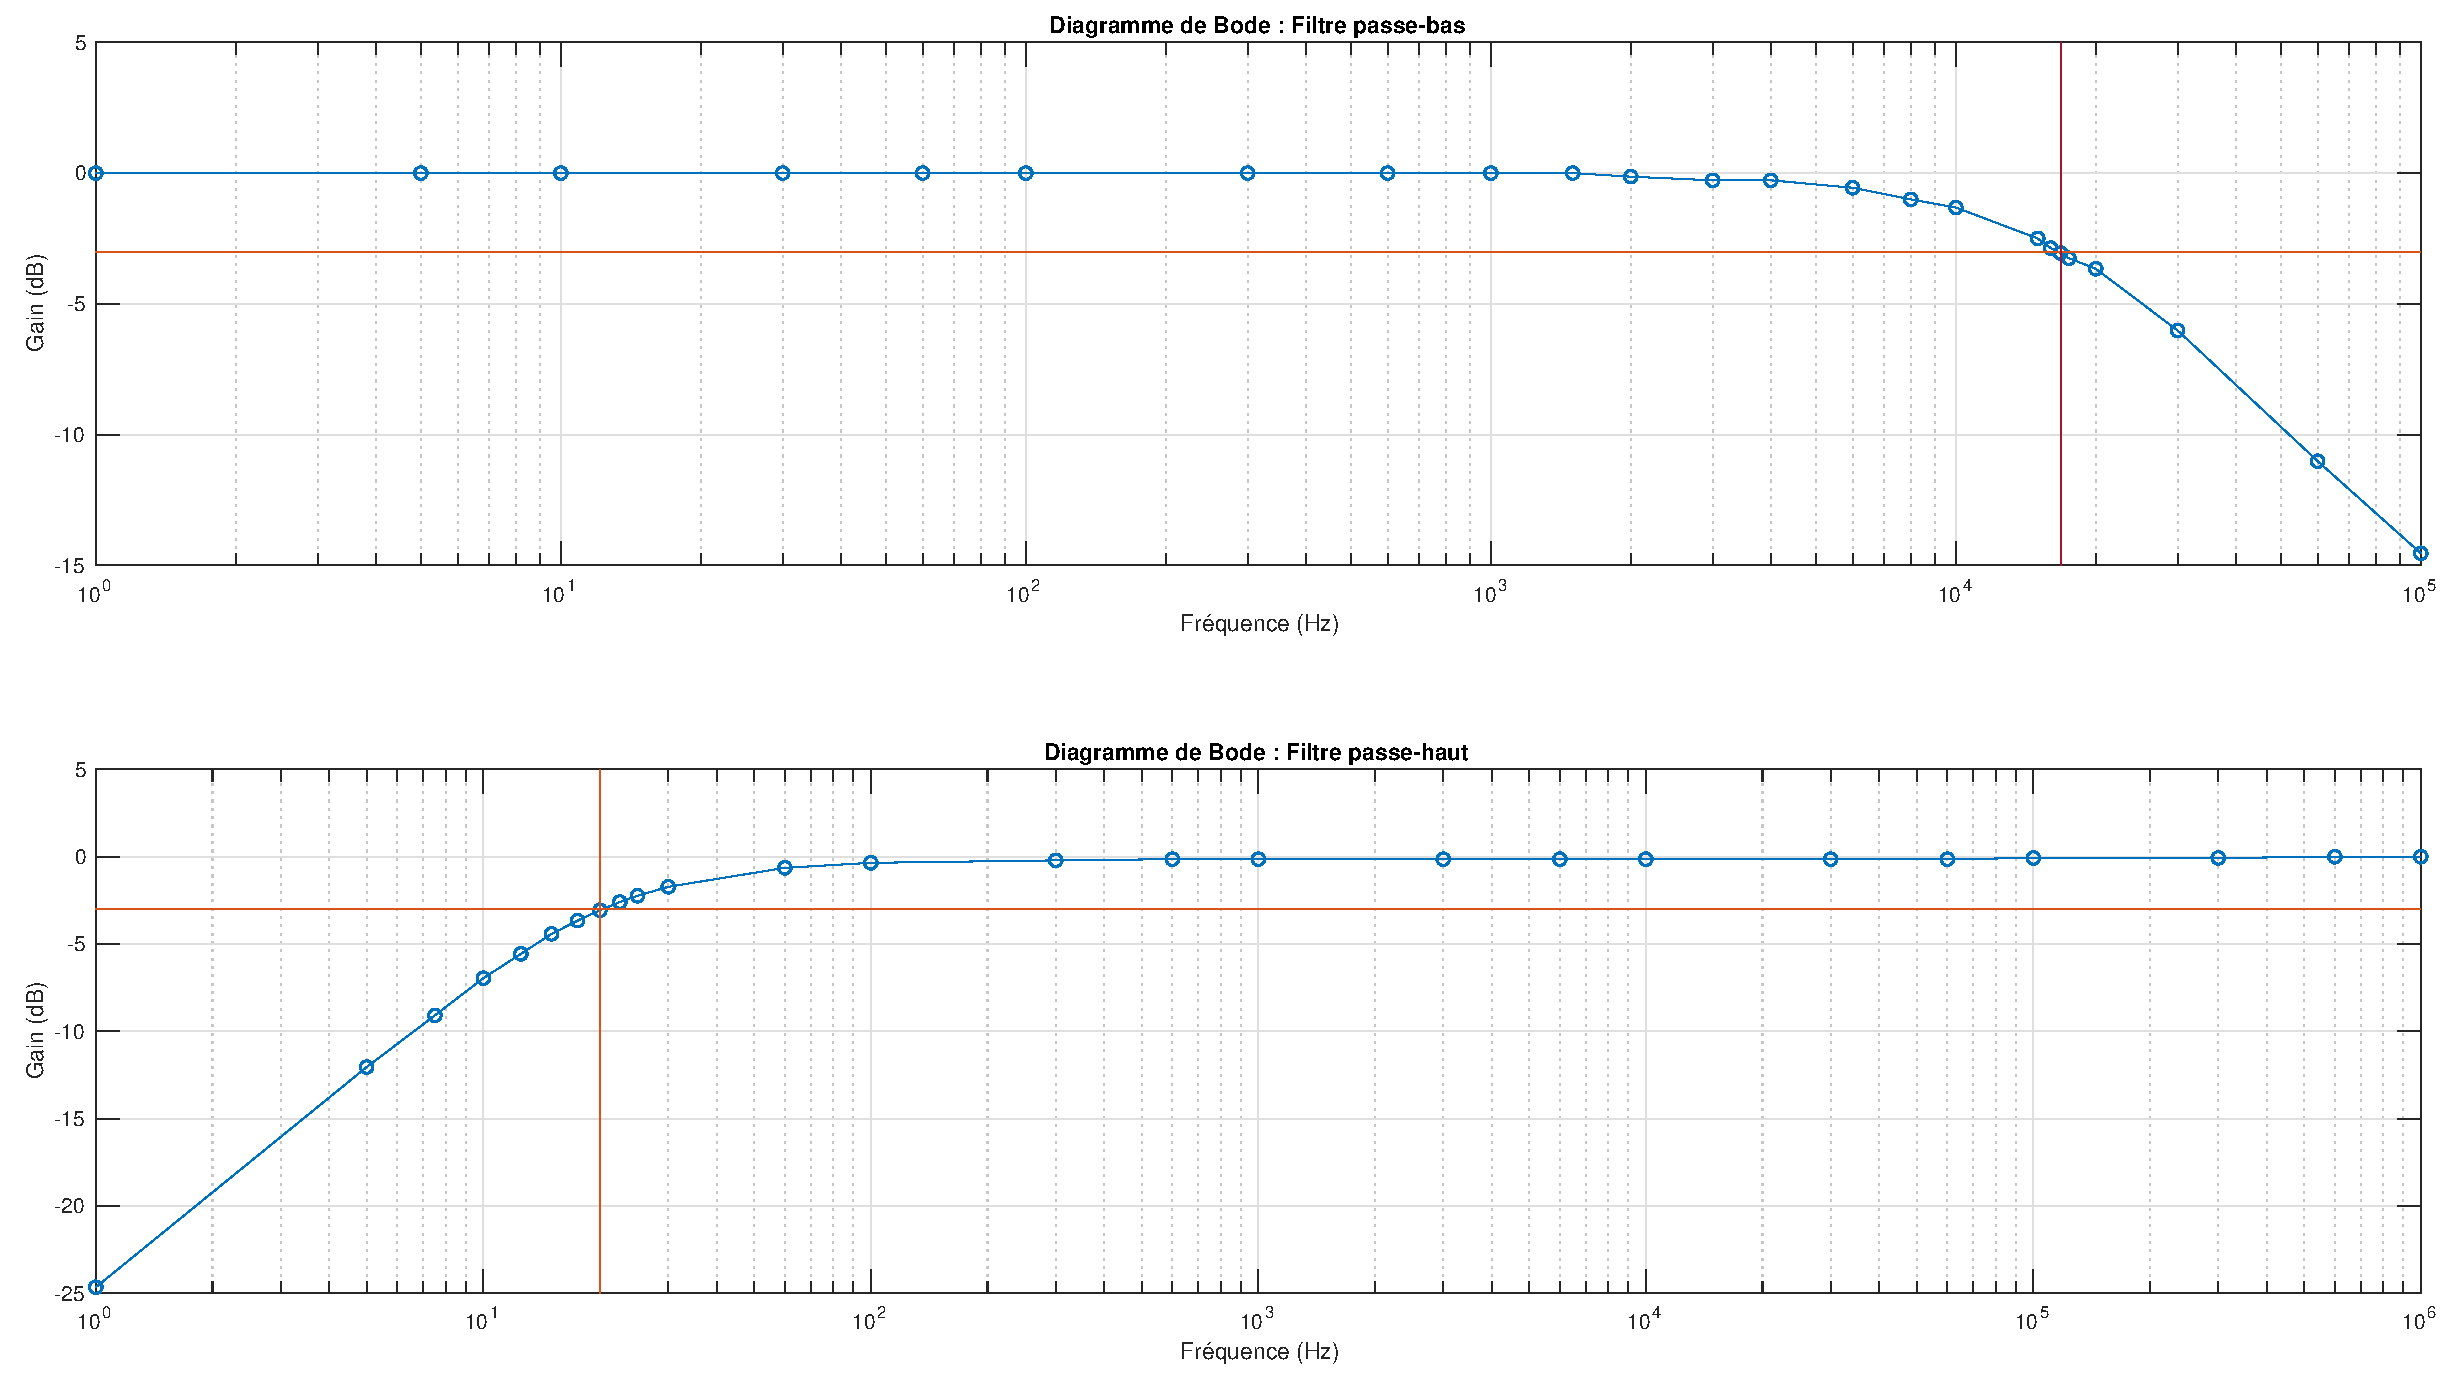
\includegraphics[width=\textwidth]{eps/bode-filtres.eps}
    \caption{Réponse fréquentielle pour les filtres passe-bas
    		 et passe-haut de l'amplificateur classe D.}
\end{figure}

\subsection{Filtre RC}

\subsection{Constante de temps du Sigma-Delta}

%%%%%%%%%%%%%%%%%%%%%%%%%%%%
\section{Analyse du circuit}
Après que les éléments aient été dimensionnée, nous avons opté pour analyser le circuit en le faisant fonctionner en régime normal et en prenant des mesures en différents points.
Ces mesures sont toujours, sauf si cité explicitement, en tension par rapport à la masse, elle même mise à la terre.

\subsection{Défaut de fabrication}
Dés le premier branchement de la carte en tension symétrique \pm\SI{25}{\volt}DC,
nous avons observé un appel de courant de \SI{200}{\milli\ampere} sur le circuit.
Cette valeur était le maximum parametré sur l'alimentation de laboratoire à notre portée.
Ce courant est trop élevé pour un amplificateur au repos, c.-à-d. sans signal d'entrée.
Il n'y a nul doute qu'un problème de connexion existe sur la carte.

Pour cerner le problème, nous avons connecté un ohmmètre entre les bornes d'alimentation : positive-négative, positive-neutre, neutre-négative.
À ces bornes nous avons mesuré respectivement une résistance de : \SI{33}{\Omega}, \SI{9}{\kilo\Omega} et \SI{9}{\kilo\Omega}.
C'est désormais déterminé et mesuré, il existe un défaut de connexion entre la borne positive et le neutre.

Une analyse bloc-par-bloc a permis de déterminer que le problème était le circuit intégré \verb|TC4428|, un double inverseur présentant un courant de fuite de \SI{100}{\milli\ampere} pour une tension d'alimentation de seulement \SI{4.3}{\volt};
ce qui est déraisonnable et en opposition avec la fiche technique du produit.
Nous en avons déduit que le composant était détruit.

Après avoir remplacé le circuit intégré \verb|TC4428|, nous avons observé que la résistance entre la borne d'alimentation positive et le neutre passait de \SI{33}{\Omega} à \SI{200}{\Omega}, ce qui n'est toujours pas acceptable.
Nous avons remplacé un second circuit intégré douteux, le \verb|L6385E|, et la résistance est passée de \SI{200}{\Omega} à \SI{19}{\kilo\Omega}; ce qui est désormais raisonnable.
Tout cela démontre que deux des circuits imprimés ont été détruits.
Nous ne savons pas déterminer l'instant auquel cela s'est produit.


%%%%%%%%%%%%%%%%%%%%%
\section*{Conclusion}
    \pdfbookmark[1]{Conclusion}{sec:conclusion}


%%%%%%%%%%%%%%%%%%
\section*{Crédits}
    \pdfbookmark[1]{Crédits}{sec:credits}
\begin{itemize}

\item Figure~\ref{fig:sigmaDelta} provenant de :\\*
Le blog officiel de Texas Instrument :
\url{https://e2e.ti.com/blogs_/archives/b/precisionhub/archive/2015/01/21/delta-sigma-adc-basics-understanding-the-delta-sigma-modulator}

\item Figure~\ref{fig:classeD} provenant de :\\*
Par Yves-Laurent (Travail personnel) [GFDL (\url{http://www.gnu.org/copyleft/fdl.html}),
CC-BY-SA-3.0 (\url{http://creativecommons.org/licenses/by-sa/3.0/})], via Wikimedia Commons

\end{itemize}

%%%%%%%%%%%%%%%%%%%%%%%%%%%%%%%%%%%%%%%%%%%
\pdfbookmark[1]{Références}{sec:references}
\bibliographystyle{unsrt}
\bibliography{ampli-classe-d}

%%%%%%%%%
\appendix
\includepdf[pagecommand=\section{Schéma du circuit DIDACTRL}]{pdf/DIDACTRL.pdf}
\includepdf[pagecommand=\section{Schéma du circuit DIDAMOS}]{pdf/DIDAMOS.pdf}
\includepdf[pagecommand=\section{Schéma du circuit DIDAMO2}]{pdf/DIDAMO2.pdf}

\end{document}
